\chapter*{Chapitre 3 : Conception et Modélisation}
\addcontentsline{toc}{chapter}{Chapitre 3 : Conception et Modélisation}
\thispagestyle{fancy}
\setcounter{section}{0}
\newpage

\section{Introduction}
La première phase du projet a été consacrée à la conception initiale, à la définition de l'architecture backend et des bases de données, ainsi qu'à la création des premiers diagrammes UML.

\section{Méthodologie Adoptée}
La méthodologie adoptée pour la conception du système s'est basée sur une approche structurée et itérative.

\subsection{Modèle en cascade}
Pour la phase de conception, nous avons adopté une approche en cascade adaptée, permettant de définir clairement les étapes successives tout en maintenant la possibilité de réviser les décisions précédentes au besoin.

\subsection{Langage UML}
Le langage UML (Unified Modeling Language) a été utilisé comme standard pour représenter graphiquement l'architecture et les interactions du système. Ce choix permet une communication claire et non ambiguë entre toutes les parties prenantes du projet.

\section{Conception}

\subsection{Identification des acteurs}
Les principaux types d'utilisateurs identifiés pour la plateforme sont :
\begin{itemize}
  \item \textbf{Apprenant Individuel :} S'inscrit, s'abonne, apprend, demande des consultations
  \item \textbf{Employé d'Entreprise :} Apprend via l'abonnement de l'entreprise, demande des consultations
  \item \textbf{Administrateur/Manager d'Entreprise :} Gère le compte de l'entreprise, les employés, les abonnements, attribue les cours, consulte les analyses
  \item \textbf{Créateur de Cours :} Conçoit et élabore le contenu des cours (modules, leçons, quiz)
  \item \textbf{Consultant/Fournisseur de Prestations :} Gère sa disponibilité, anime les sessions via la plateforme de réunion
  \item \textbf{Agent de Support Plateforme :} Assiste les utilisateurs pour les problèmes liés à la plateforme et les questions-réponses
  \item \textbf{Administrateur de la Plateforme :} Supervise l'ensemble de la plateforme, les utilisateurs, le contenu, les paramètres
\end{itemize}

\subsection{Identification des messages}
La plateforme e-learning conçue repose sur les fonctionnalités essentielles suivantes :
\begin{itemize}
    \item \textbf{E-Learning :}
    \begin{itemize}
        \item Catalogue de cours (filtrable, consultable)
        \item Modules, Leçons (vidéo, basées sur des images)
        \item Quiz et Évaluations
        \item Suivi de la Progression
        \item Certificats de Réussite
        \item Support Multilingue (EN/FR)
        \item Paramètres Utilisateur et Entreprise
    \end{itemize}
    \item \textbf{Consultation et Prestation :}
    \begin{itemize}
        \item Navigation des services
        \item Profils des consultants et disponibilité
        \item Système de réservation/demande
        \item Intégration API avec la plateforme de réunion personnalisée
        \item Facturation des sessions
    \end{itemize}
    \item \textbf{Monétisation :}
    \begin{itemize}
        \item Abonnements pour utilisateurs individuels (accès illimité)
        \item Abonnements pour entreprises (par utilisateur)
        \item Réductions et Démos
    \end{itemize}
\end{itemize}

\subsection{Les diagrammes de cas d'utilisation}
Les diagrammes de cas d'utilisation ont permis de représenter visuellement les interactions entre les acteurs et le système.

\begin{figure}[p]
  \centering
  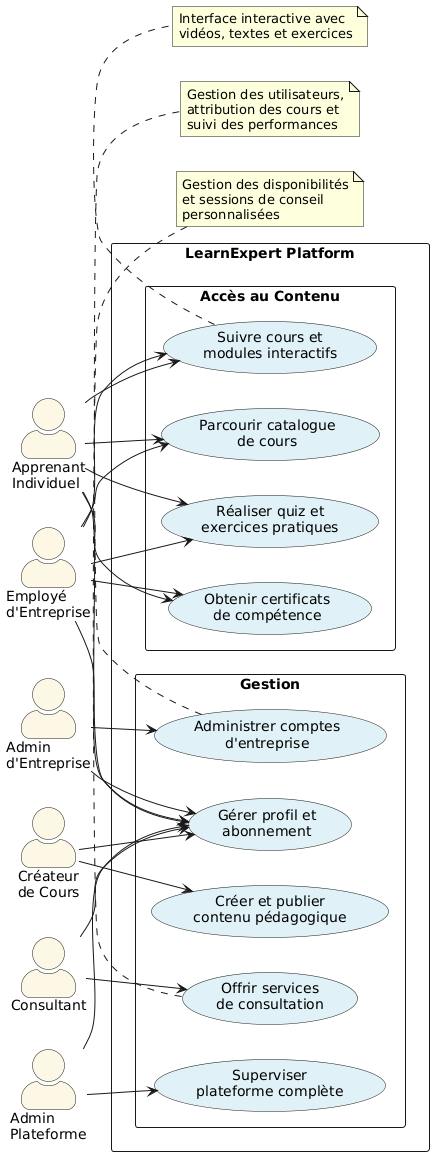
\includegraphics[width=0.52\textwidth,keepaspectratio]{images/usecase_diagram.png}
  \caption{\textbf{Diagramme de cas d'utilisation} montrant les principales fonctionnalités accessibles par les acteurs.}
  \label{fig:usecase_diagram}
\end{figure}
\clearpage

\subsection{Les diagrammes de séquence}
Les diagrammes de séquence ont permis d'illustrer les interactions temporelles entre les différents composants du système pour des scénarios clés.

Pour illustrer le fonctionnement de l'architecture, voici un exemple de flux de communication entre les services pour un scénario d'inscription et d'abonnement :
\begin{enumerate}
  \item \textbf{Client (Next.js)} $\rightarrow$ \textbf{Passerelle API (Nginx)} $\rightarrow$ \textbf{Service IAM} (Création de l'utilisateur)
  \item \textbf{Service IAM} $\rightarrow$ \textbf{Kafka} (Publie `UserRegisteredEvent`)
  \item \textbf{Service de Notification} (Consomme l'événement) $\rightarrow$ Envoie un Email de Bienvenue
  \item \textbf{Client} $\rightarrow$ \textbf{Passerelle API} $\rightarrow$ \textbf{Service de Facturation} (Demande d'abonnement)
  \item \textbf{Service de Facturation} $\rightarrow$ Passerelle de Paiement et Mise à jour de la BD interne
  \item \textbf{Service de Facturation} $\rightarrow$ \textbf{Kafka} (Publie `SubscriptionActivatedEvent`)
  \item \textbf{Service IAM} (Consomme, met à jour le statut utilisateur) \& \textbf{Service de Notification} (Consomme, envoie une confirmation)
\end{enumerate}

\begin{figure}[p]
  \centering
  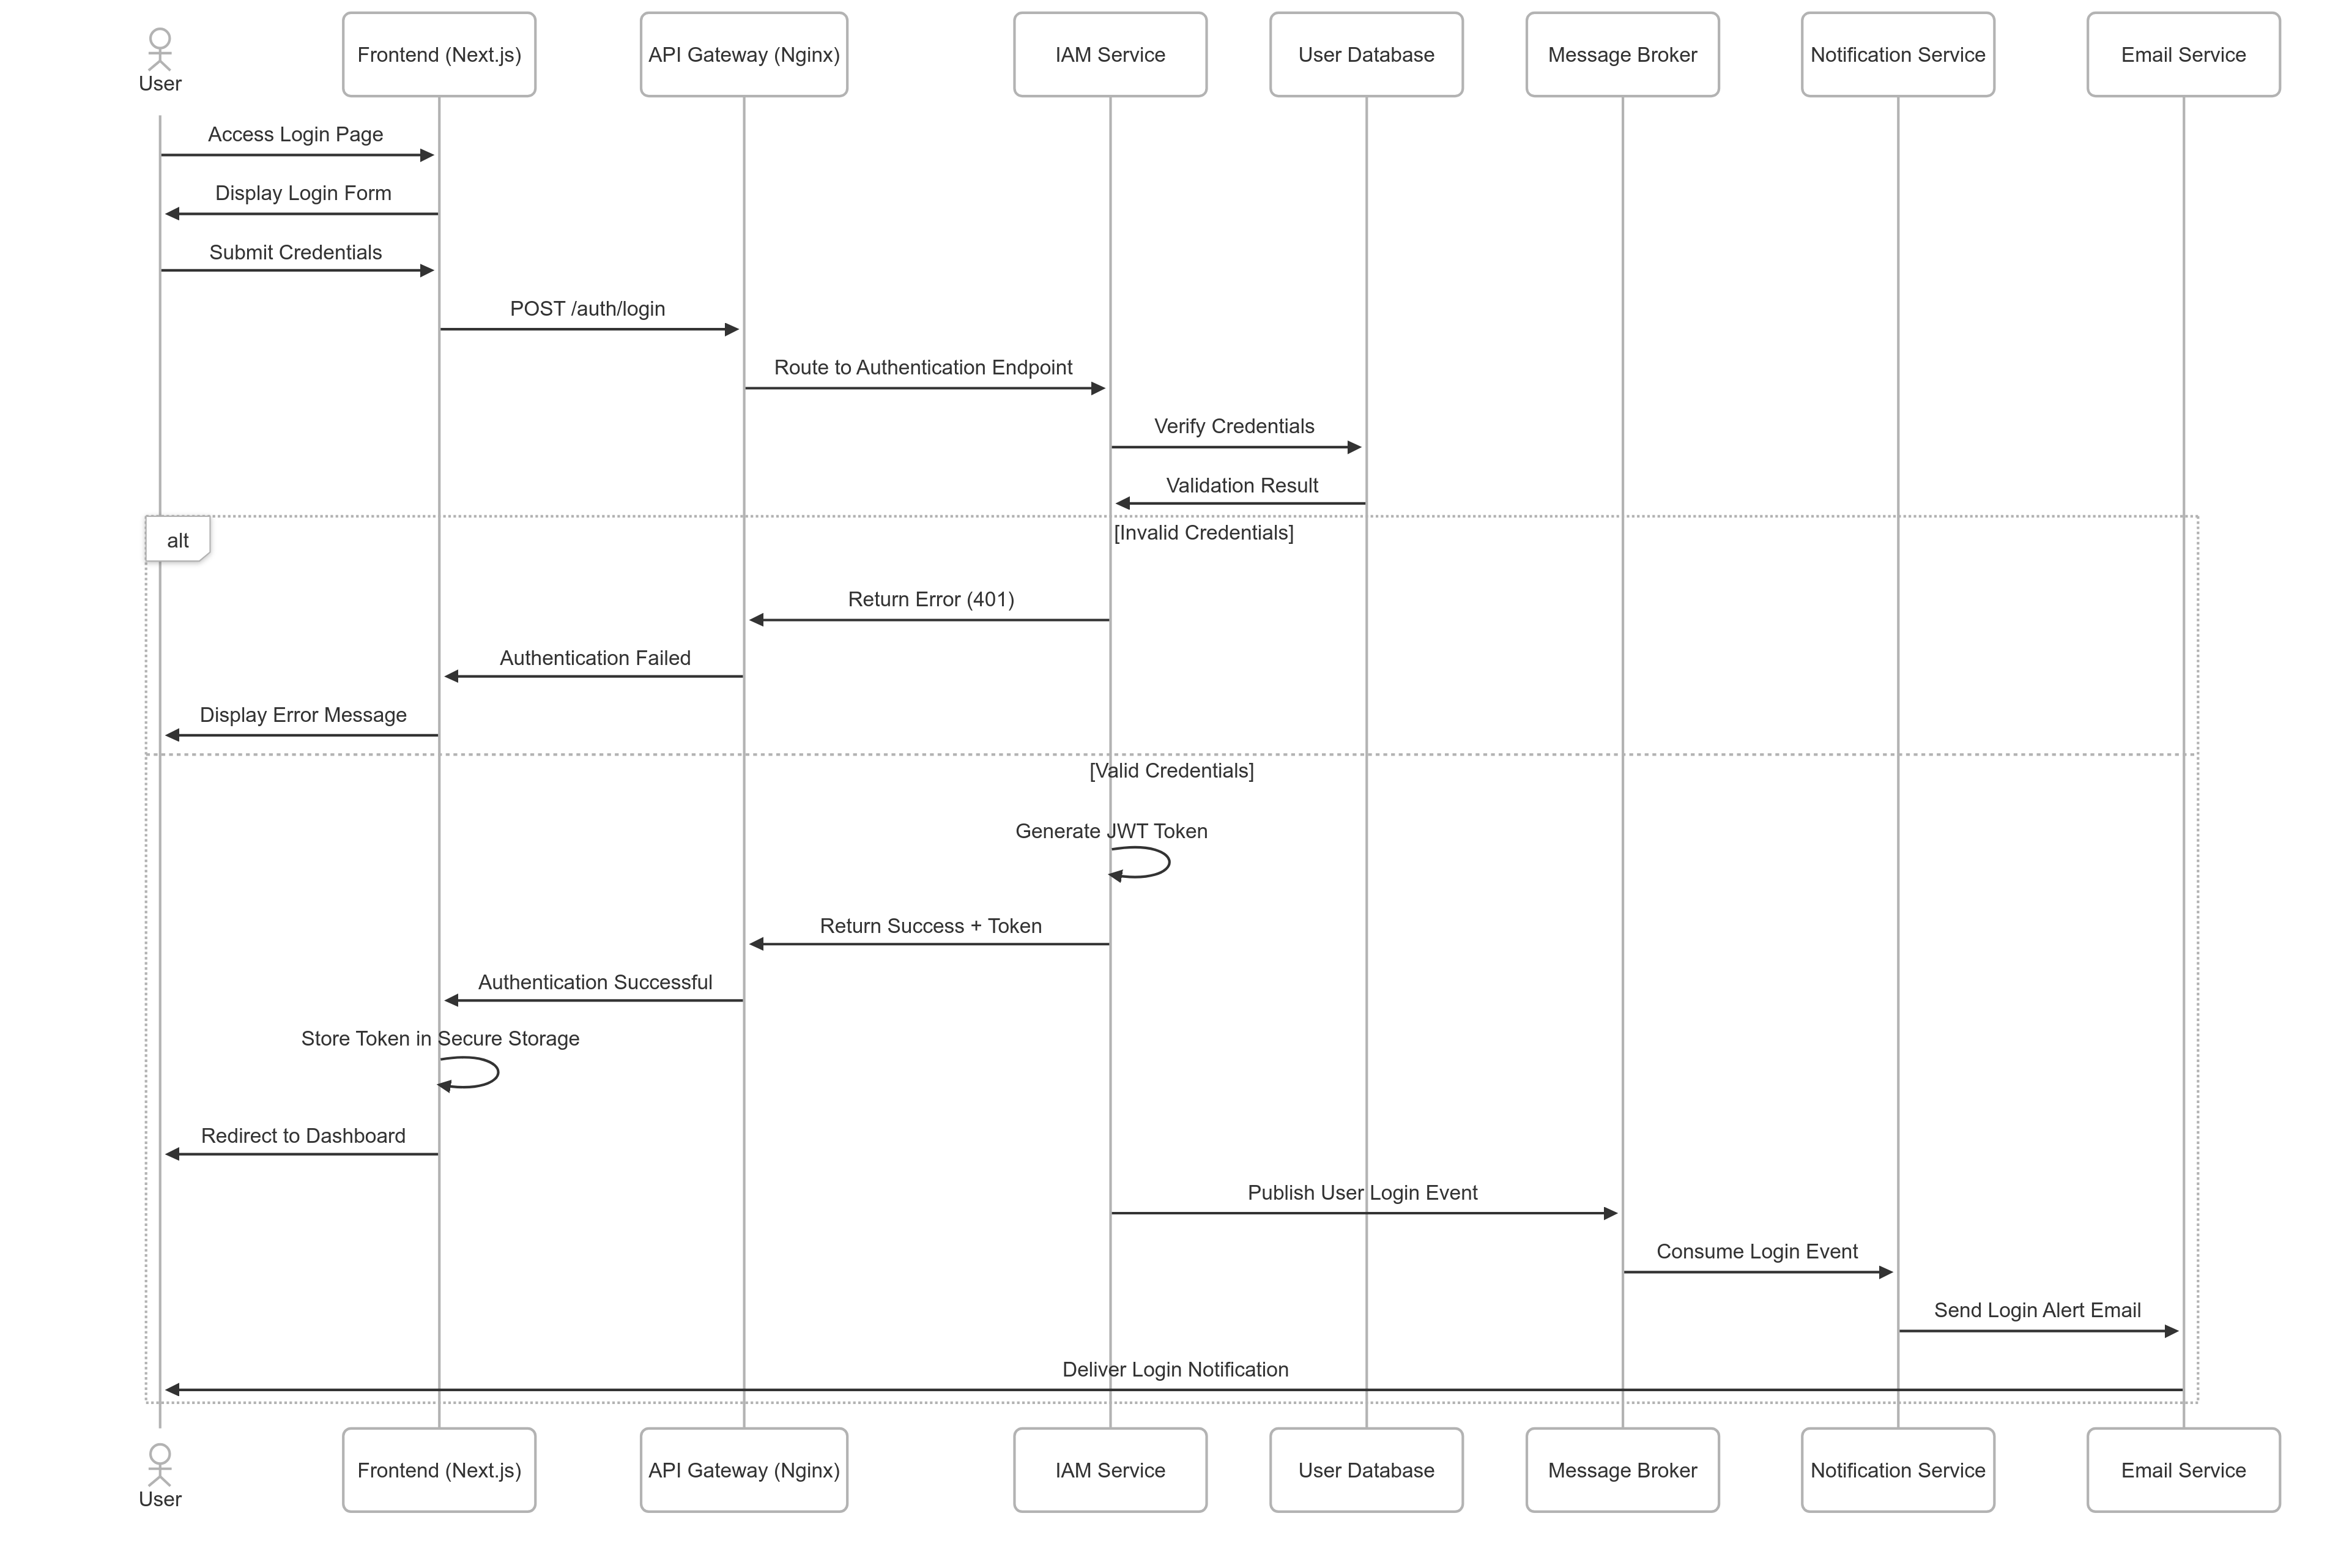
\includegraphics[width=0.9\textwidth,keepaspectratio]{images/sequence_diagram.png}
  \caption{\textbf{Diagramme de séquence} illustrant le processus d'authentification et de notification.}
  \label{fig:sequence_diagram}
\end{figure}
\clearpage

\subsection{Le diagramme de classes}
Le diagramme de classes a été élaboré pour représenter les principales entités du système et leurs relations.

\begin{figure}[p]
  \centering
  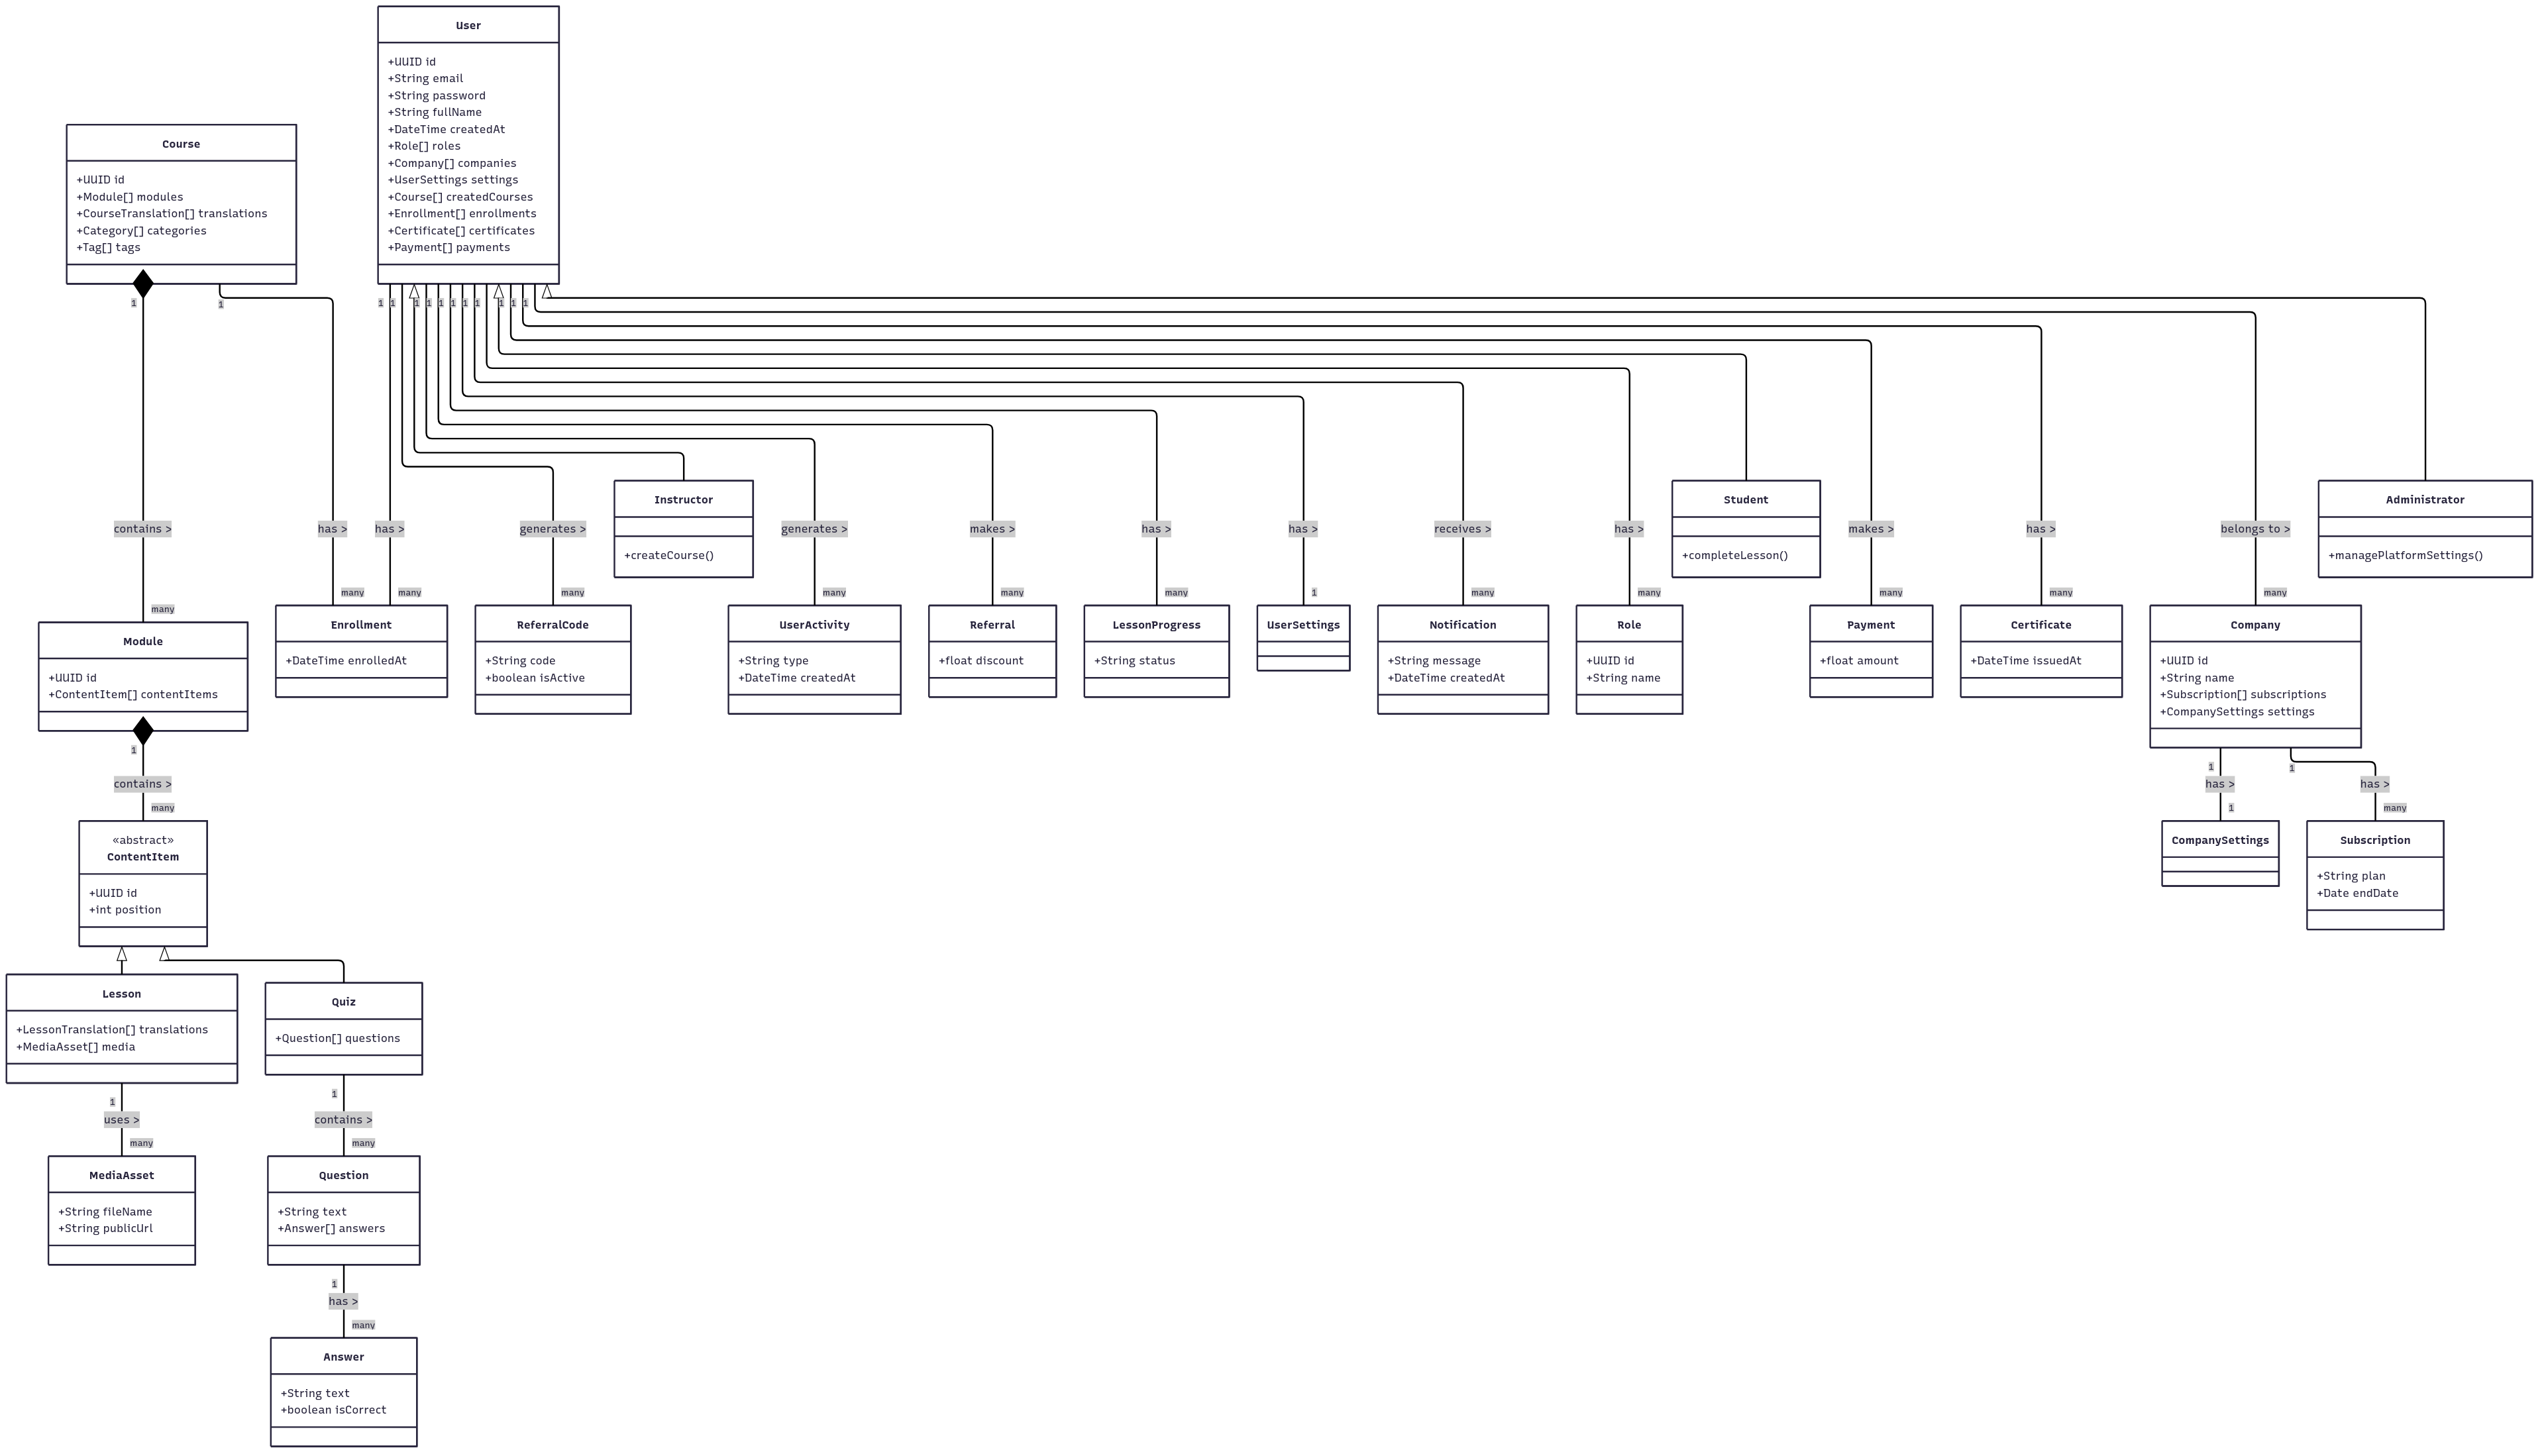
\includegraphics[width=0.9\textwidth,keepaspectratio]{week_1_img/class_diagrame.png}
  \caption{\textbf{Diagramme de classes} de la plateforme e-learning montrant les principales entités et leurs relations.}
  \label{fig:class_diagram}
\end{figure}

Ce diagramme illustre les relations entre les différentes entités du système, comme les utilisateurs, les cours, les modules, les leçons, les abonnements et les services de consultation. Les cardinalités et les types de relations (composition, agrégation, héritage) ont été définies pour refléter précisément la structure du modèle de données.
\clearpage

\section{Architecture Adoptée}

L'architecture envisagée pour la plateforme repose sur une approche de microservices, justifiée par plusieurs avantages clés :
\begin{itemize}
  \item \textbf{Scalabilité :} Mise à l'échelle indépendante des services individuels selon les besoins
  \item \textbf{Maintenabilité :} Possibilité de modifier des parties spécifiques sans impacter l'ensemble du système
  \item \textbf{Résilience :} Limitation de l'impact des défaillances à des services spécifiques
  \item \textbf{Autonomie des Équipes :} Développement, tests et déploiement indépendants par différentes équipes
  \item \textbf{Flexibilité Technologique :} Utilisation des technologies les plus adaptées pour chaque service
\end{itemize}

\subsection{Pile Technologique}
La pile technologique définie pour le développement comprend :
\begin{itemize}
  \item \textbf{Frontend :} Next.js (React)
  \item \textbf{Microservices Backend :}
    \begin{itemize}
      \item Go (pour les services critiques en performance et concurrents comme les Notifications, le backend de la plateforme de réunion)
      \item Python avec FastAPI (pour les services gourmands en données, développement rapide d'API, par exemple, Catalogue de Cours, Facturation)
      \item Node.js avec Express (TypeScript) (pour les opérations I/O intensives, interaction Supabase, par exemple, IAM, Gestion des Médias)
    \end{itemize}
  \item \textbf{Bases de Données :}
    \begin{itemize}
      \item PostgreSQL (stockage relationnel principal pour la plupart des services)
      \item Supabase (pour l'Authentification, le Stockage, et son Postgres géré pour des services spécifiques)
    \end{itemize}
  \item \textbf{Passerelle API :} Nginx (en tant que reverse proxy et passerelle)
  \item \textbf{Broker de Messages :} Apache Kafka (pour une gestion d'événements asynchrones robuste et scalable)
  \item \textbf{Conteneurisation et Orchestration :} Docker (Kubernetes serait une étape logique suivante pour l'orchestration)
\end{itemize}

\subsection{Modèles de Données des Services}
Dans le cadre de cette première phase, des modèles de données préliminaires ont été conçus pour chacun des services identifiés. Voici quelques exemples des structures de données principales :

\subsubsection{Service IAM (Identity and Access Management)}
\begin{figure}[p]
  \centering
  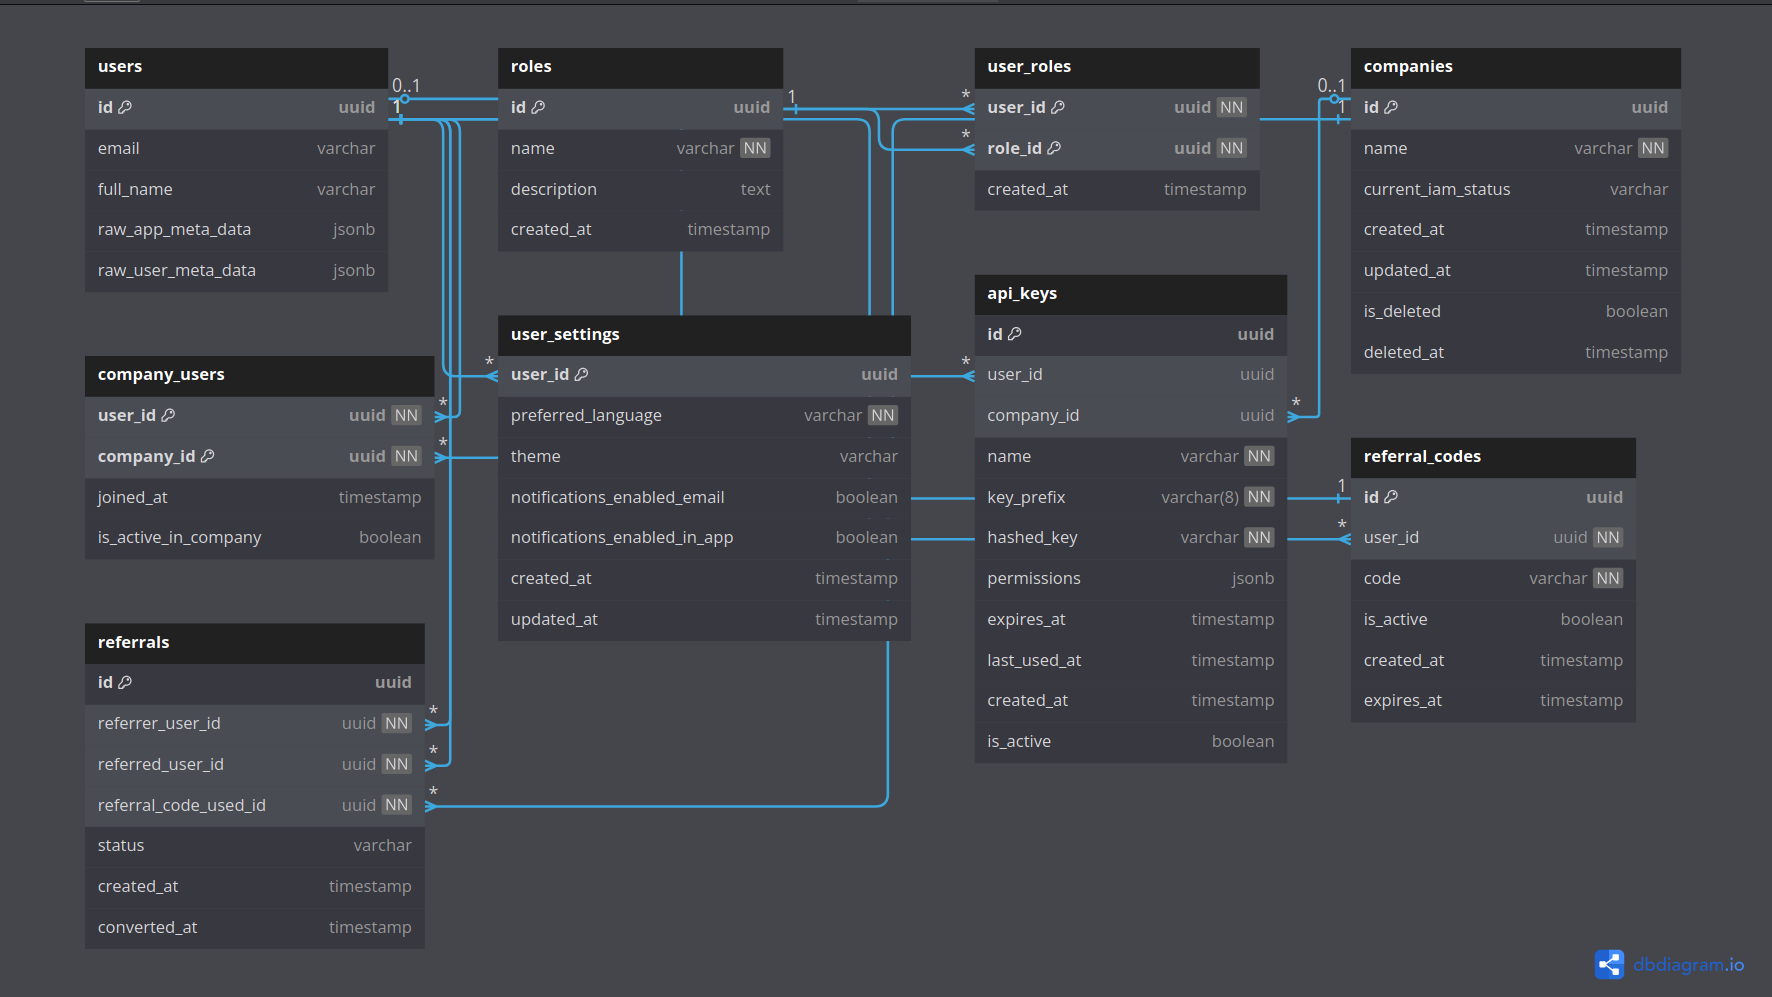
\includegraphics[width=0.8\textwidth,keepaspectratio]{week_1_img/services_db_screanshots/Screenshot 2025-06-06 at 15-08-36 IAM_Service.pdf.png}
  \caption{\textbf{Modèle de données du service IAM} pour la gestion des utilisateurs et des autorisations.}
  \label{fig:iam_service}
\end{figure}

\vspace{5pt}
\small
\paragraph{Points clés du modèle IAM :}
\begin{itemize}[leftmargin=*,noitemsep,topsep=0pt]
  \item \textbf{Gestion centralisée des utilisateurs} avec tables dédiées aux utilisateurs, rôles et permissions
  \item \textbf{Support multi-tenant} via la table des entreprises (companies)
  \item \textbf{Système de référence} permettant le suivi des recommandations et affiliations
  \item \textbf{Paramètres utilisateurs} stockés de manière structurée pour personnaliser l'expérience
  \item \textbf{Jetons d'authentification} permettant une gestion sécurisée des sessions
\end{itemize}
\normalsize
\clearpage

\subsubsection{Service de Contenu}
\begin{figure}[p]
  \centering
  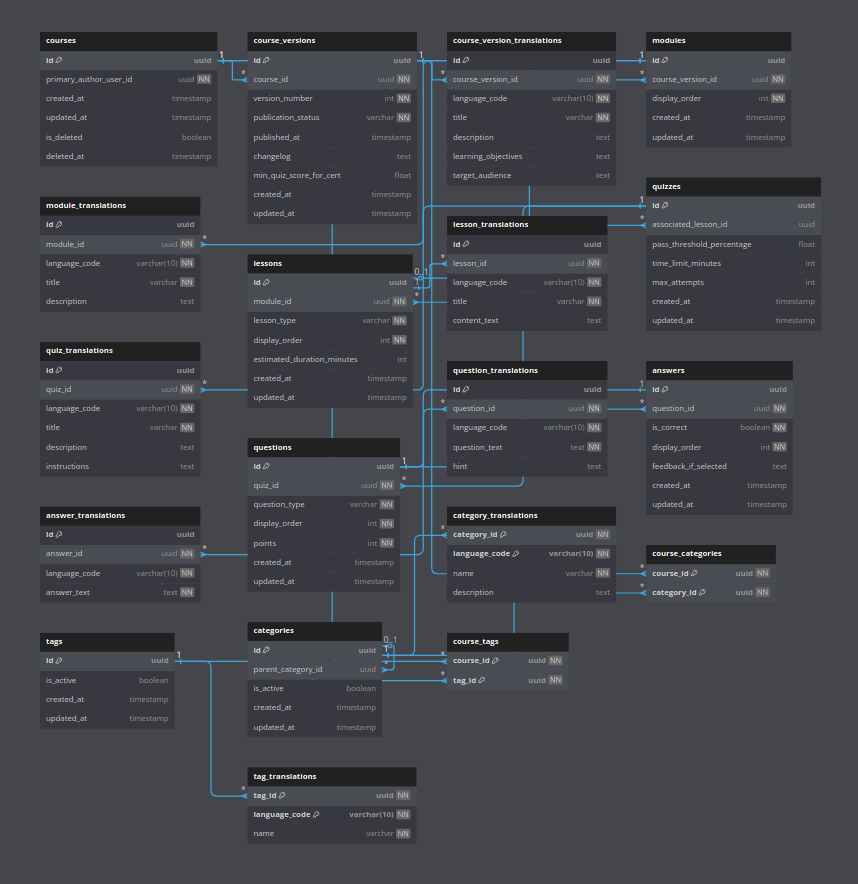
\includegraphics[width=0.8\textwidth,keepaspectratio]{week_1_img/services_db_screanshots/Screenshot 2025-06-06 at 15-07-51 Content_Service.pdf.png}
  \caption{\textbf{Modèle de données du service de contenu} pour la gestion des cours et ressources pédagogiques.}
  \label{fig:content_service}
\end{figure}

\vspace{5pt}
\small
\paragraph{Points clés du service de Contenu :}
\begin{itemize}[leftmargin=*,noitemsep,topsep=0pt]
  \item \textbf{Structure hiérarchique} des cours, modules et leçons
  \item \textbf{Support multimédia} avec gestion des vidéos, documents et quizz
  \item \textbf{Métadonnées riches} pour faciliter la recherche et la catégorisation
  \item \textbf{Gestion des versions} permettant la mise à jour du contenu sans perte d'historique
  \item \textbf{Support multilingue} pour internationaliser le contenu pédagogique
\end{itemize}
\normalsize
\clearpage

\subsubsection{Service de Facturation et d'Abonnement}
\begin{figure}[p]
  \centering
  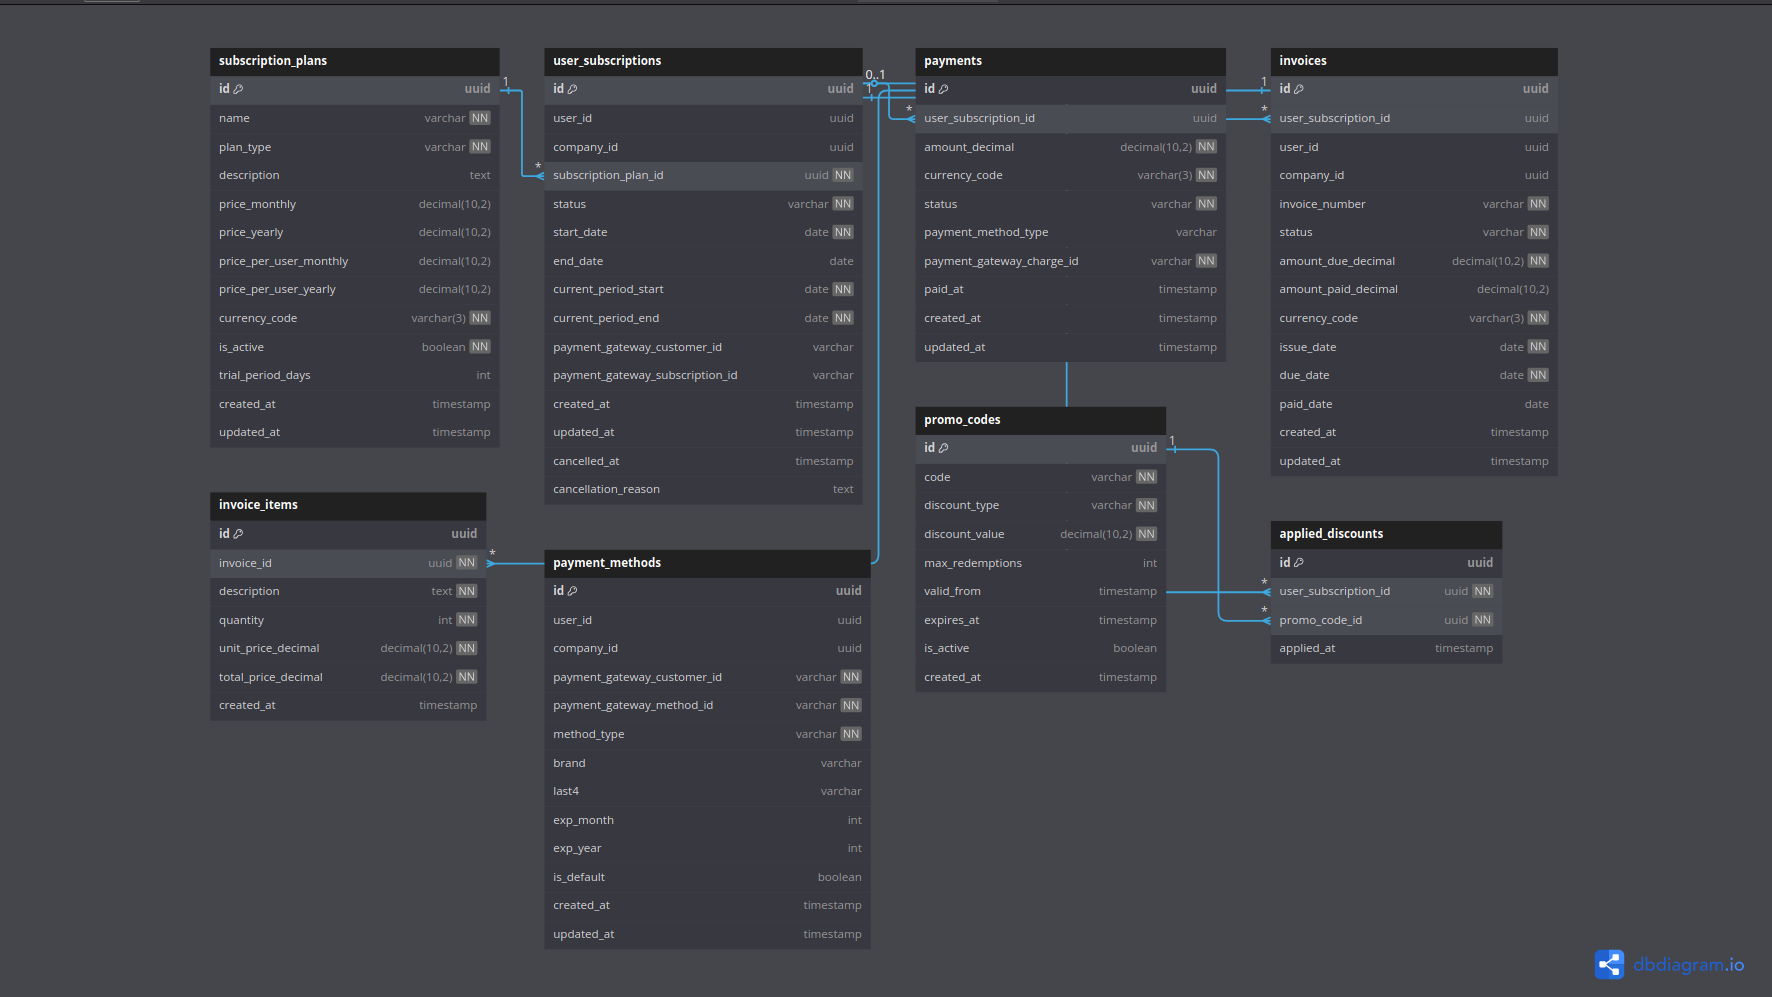
\includegraphics[width=0.8\textwidth,keepaspectratio]{week_1_img/services_db_screanshots/Screenshot 2025-06-06 at 15-05-28 Billing_and_Subscription_Service.pdf.png}
  \caption{\textbf{Modèle de données du service de facturation} pour la gestion des abonnements et des paiements.}
  \label{fig:billing_service}
\end{figure}

\vspace{5pt}
\small
\paragraph{Points clés du service de Facturation :}
\begin{itemize}[leftmargin=*,noitemsep,topsep=0pt]
  \item \textbf{Gestion des plans d'abonnement} avec différents niveaux de service
  \item \textbf{Suivi des factures et paiements} pour les utilisateurs individuels et entreprises
  \item \textbf{Support des promotions et réductions} temporaires ou permanentes
  \item \textbf{Historique de facturation} complet pour analyses financières
  \item \textbf{Intégration} avec les passerelles de paiement externes
\end{itemize}
\normalsize
\clearpage

\subsubsection{Service de Certification}
\begin{figure}[p]
  \centering
  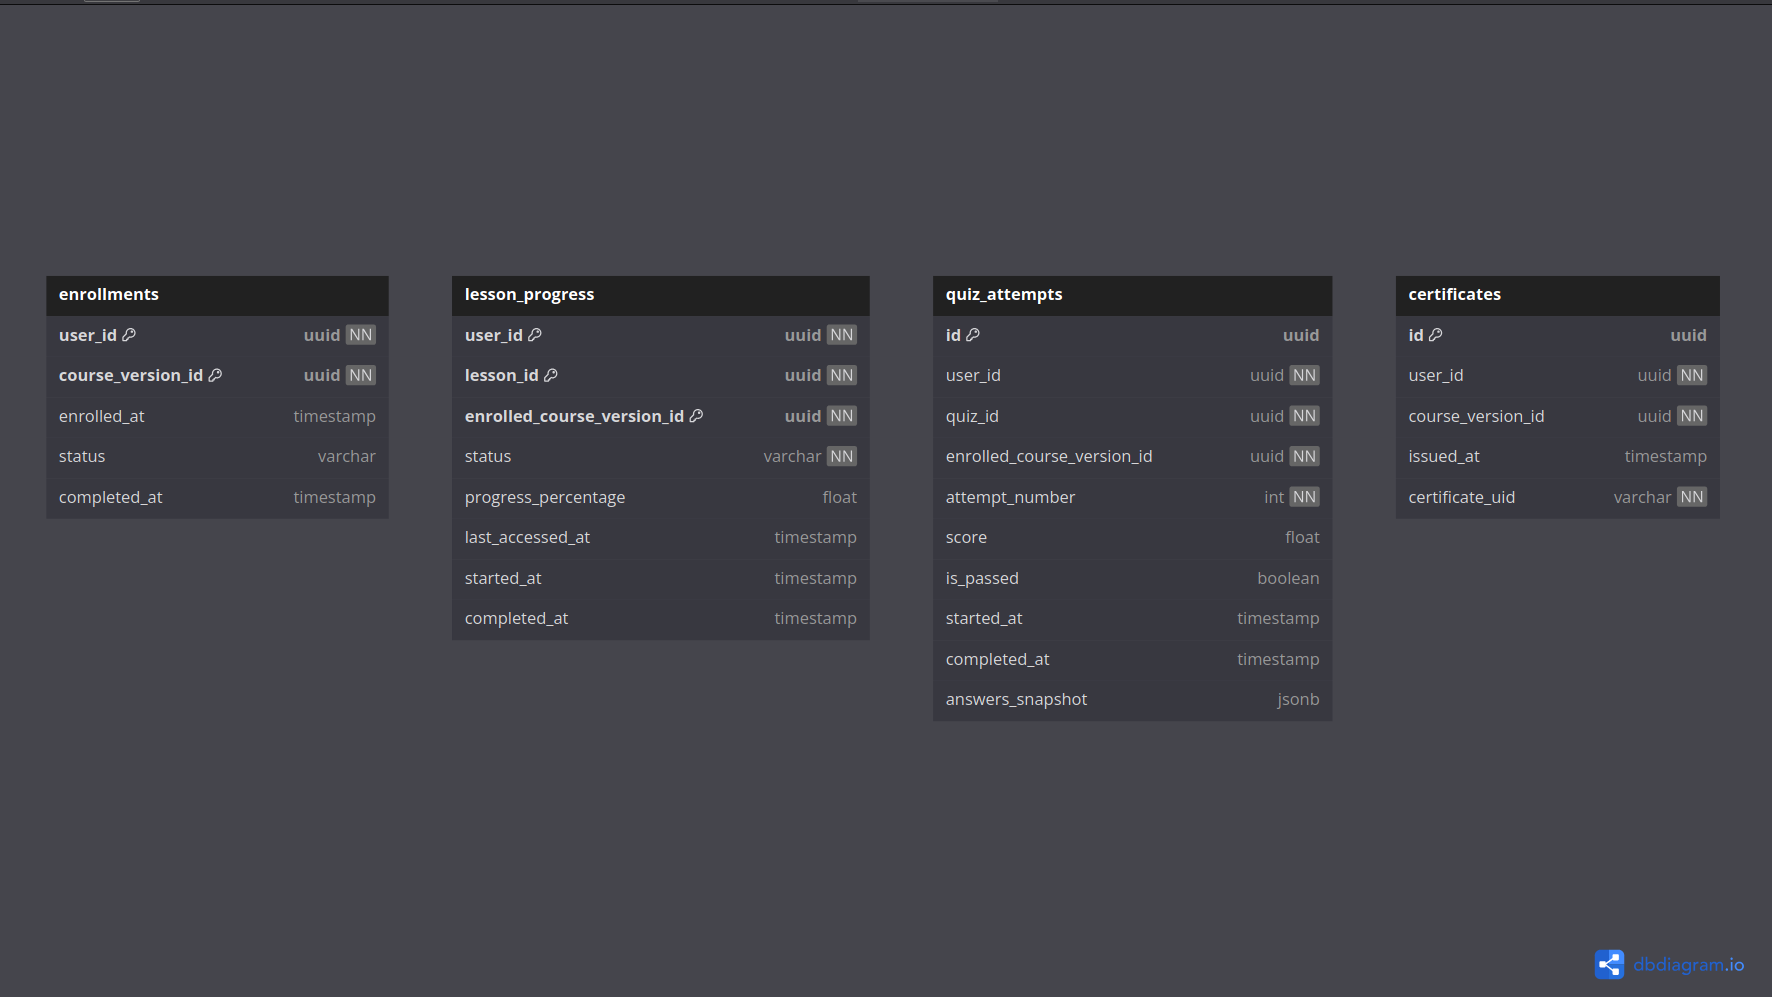
\includegraphics[width=0.8\textwidth,keepaspectratio]{week_1_img/services_db_screanshots/Screenshot 2025-06-06 at 15-05-53 Certification_Service.pdf.png}
  \caption{\textbf{Modèle de données du service de certification} pour la délivrance et la validation des certificats.}
  \label{fig:certification_service}
\end{figure}

\vspace{5pt}
\small
\paragraph{Points clés du service de Certification :}
\begin{itemize}[leftmargin=*,noitemsep,topsep=0pt]
  \item \textbf{Création de certificats} à l'achèvement des cours et modules
  \item \textbf{Validation et vérification} des compétences acquises
  \item \textbf{Badges et récompenses} pour motiver les apprenants
  \item \textbf{Système de validation externe} permettant aux entreprises de vérifier l'authenticité
  \item \textbf{Historique des certifications} pour chaque utilisateur
\end{itemize}
\normalsize
\clearpage

\subsubsection{Service d'Analytique et Reporting}
\begin{figure}[p]
  \centering
  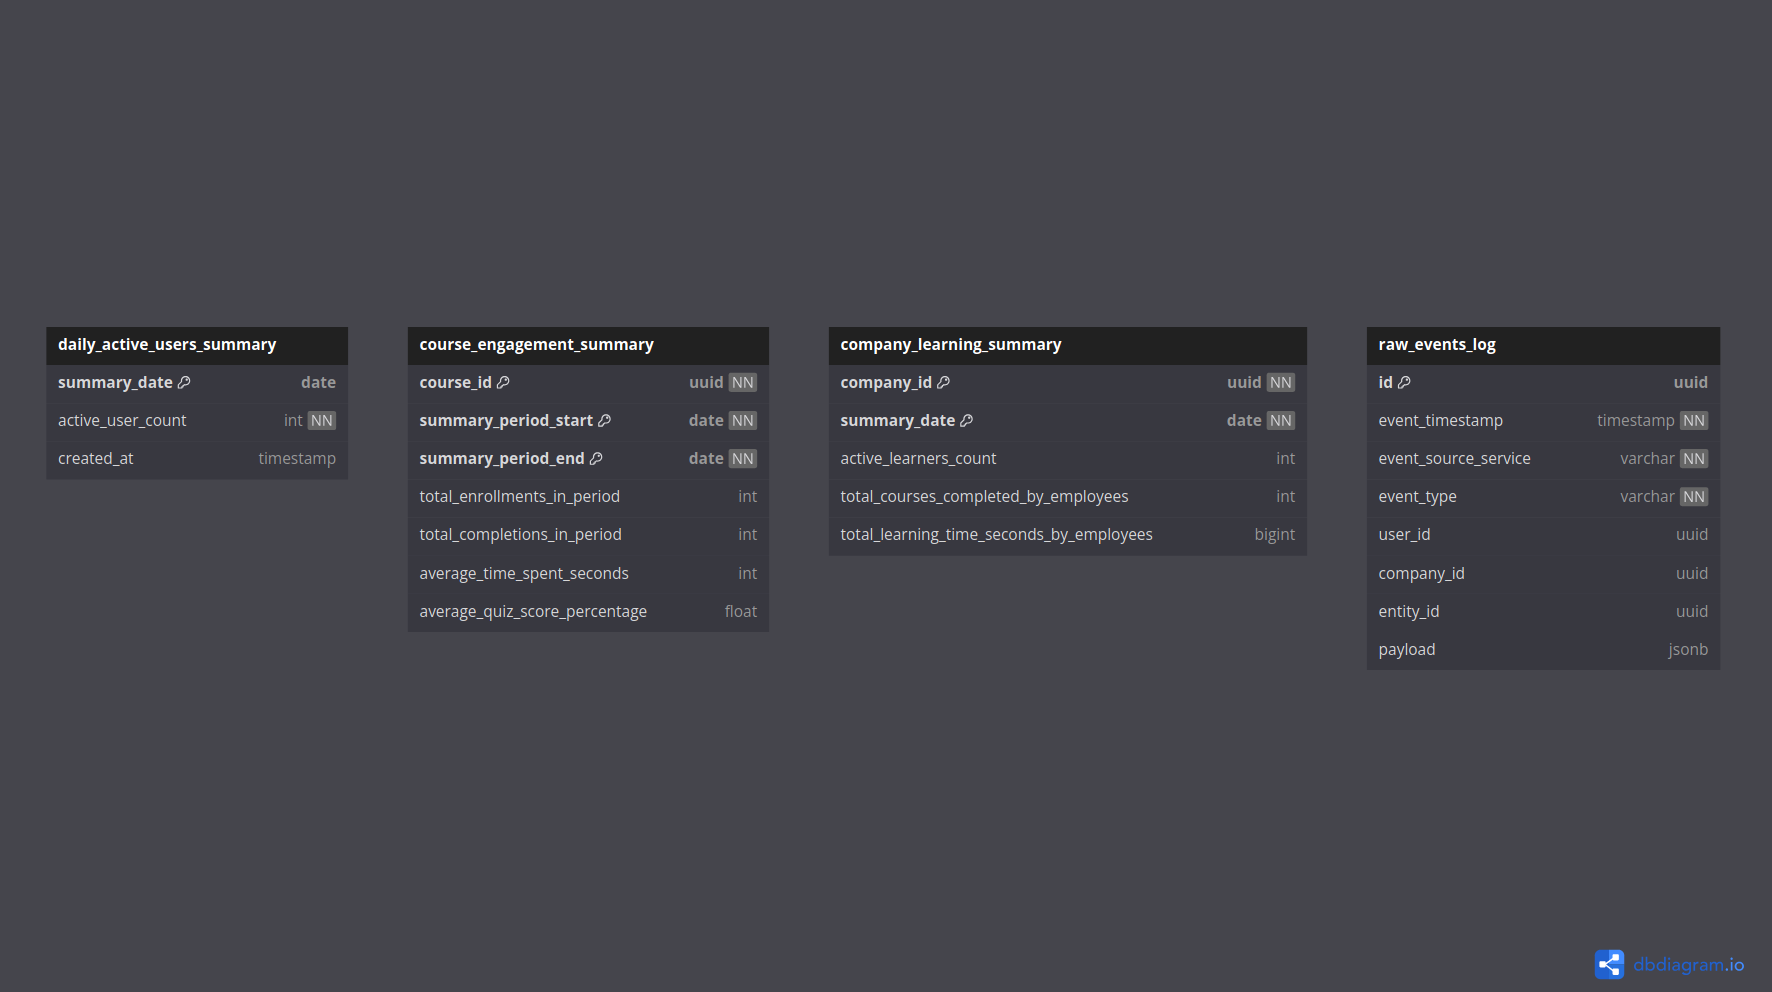
\includegraphics[width=0.8\textwidth,keepaspectratio]{week_1_img/services_db_screanshots/Screenshot 2025-06-06 at 15-04-59 Analytics_and_Reporting_Service.pdf.png}
  \caption{\textbf{Modèle de données du service d'analytique} pour le suivi des performances et la génération de rapports.}
  \label{fig:analytics_service}
\end{figure}

\vspace{5pt}
\small
\paragraph{Points clés du service d'Analytique :}
\begin{itemize}[leftmargin=*,noitemsep,topsep=0pt]
  \item \textbf{Collecte de données d'utilisation} sur toutes les interactions utilisateurs
  \item \textbf{Métriques de performance} pour les cours et modules
  \item \textbf{Rapports personnalisés} pour les administrateurs et entreprises
  \item \textbf{Tableaux de bord en temps réel} pour le suivi des indicateurs clés
  \item \textbf{Système d'alerte} pour identifier les anomalies ou opportunités
\end{itemize}
\normalsize
\clearpage

\subsubsection{Service de Feedback}
\begin{figure}[p]
  \centering
  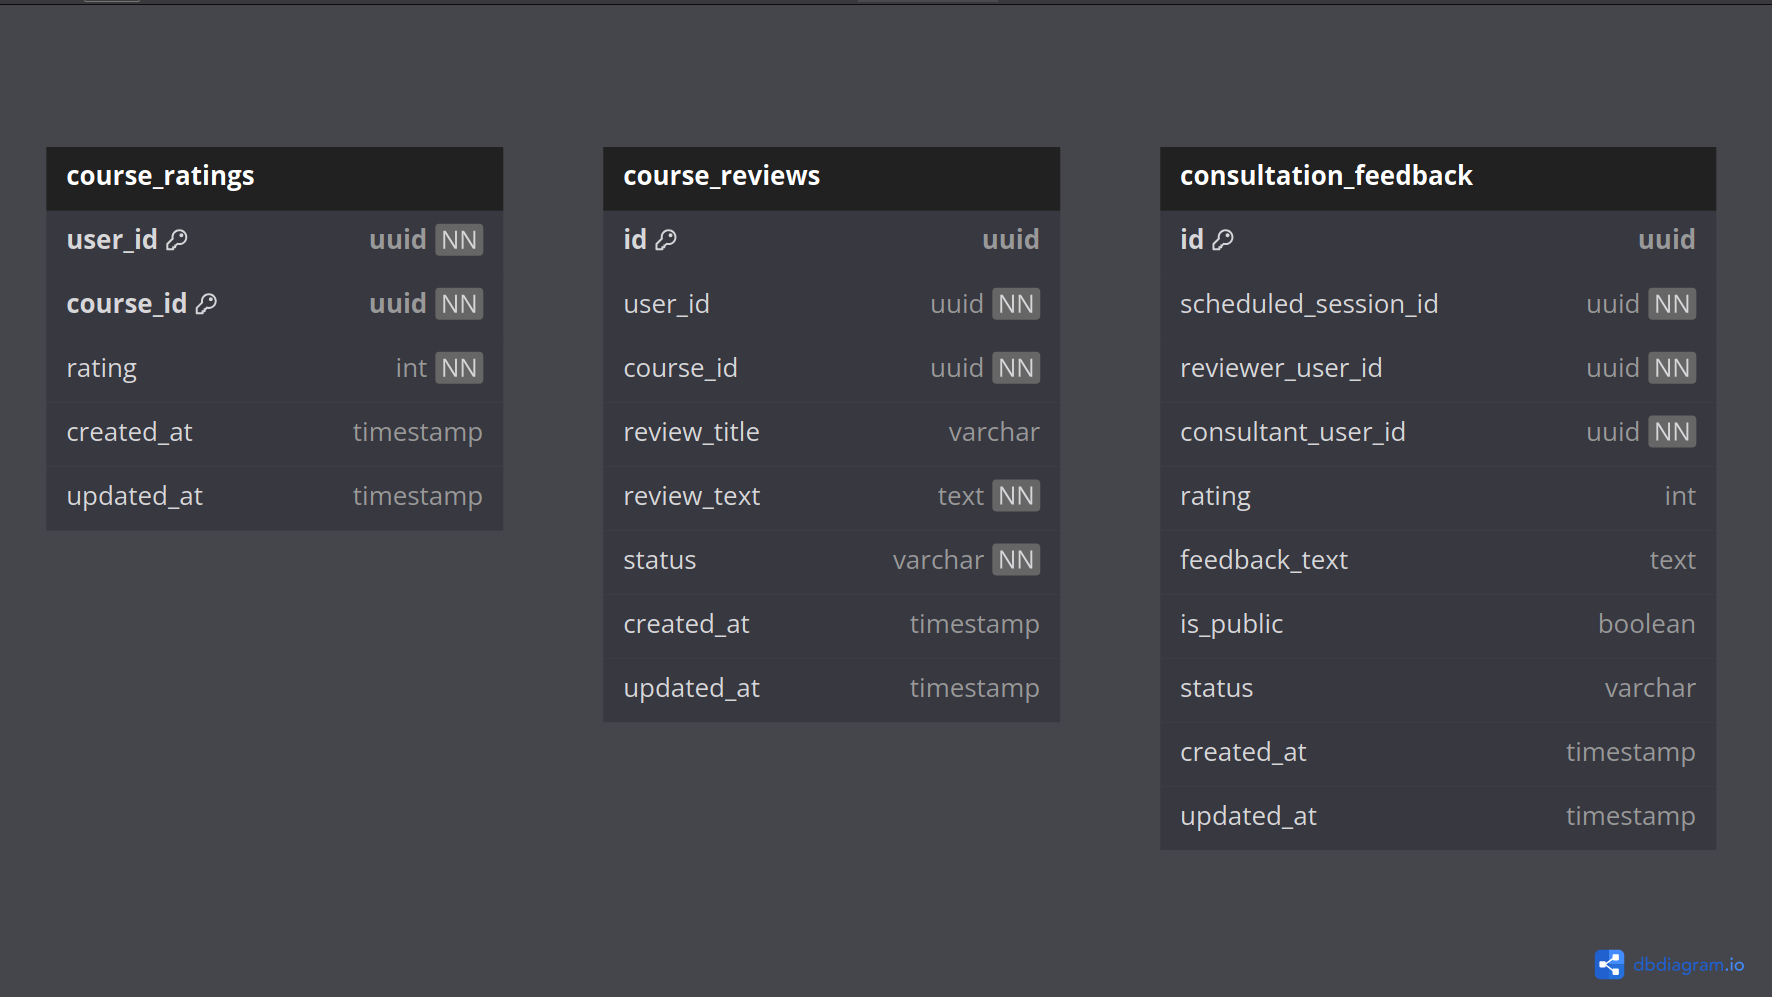
\includegraphics[width=0.8\textwidth,keepaspectratio]{week_1_img/services_db_screanshots/Screenshot 2025-06-06 at 15-08-00 Feedback_Service.pdf.png}
  \caption{\textbf{Modèle de données du service de feedback} pour la collecte et la gestion des retours utilisateurs.}
  \label{fig:feedback_service}
\end{figure}

\vspace{5pt}
\small
\paragraph{Points clés du service de Feedback :}
\begin{itemize}[leftmargin=*,noitemsep,topsep=0pt]
  \item \textbf{Évaluations et avis} sur les cours et modules
  \item \textbf{Système de notation} permettant une évaluation quantitative
  \item \textbf{Commentaires et suggestions} pour améliorer le contenu
  \item \textbf{Analyse de sentiment} sur les retours textuels
  \item \textbf{Gestion des signalements} pour modérer les contenus inappropriés
\end{itemize}
\normalsize
\clearpage

\subsubsection{Service de Notification}
\begin{figure}[p]
  \centering
  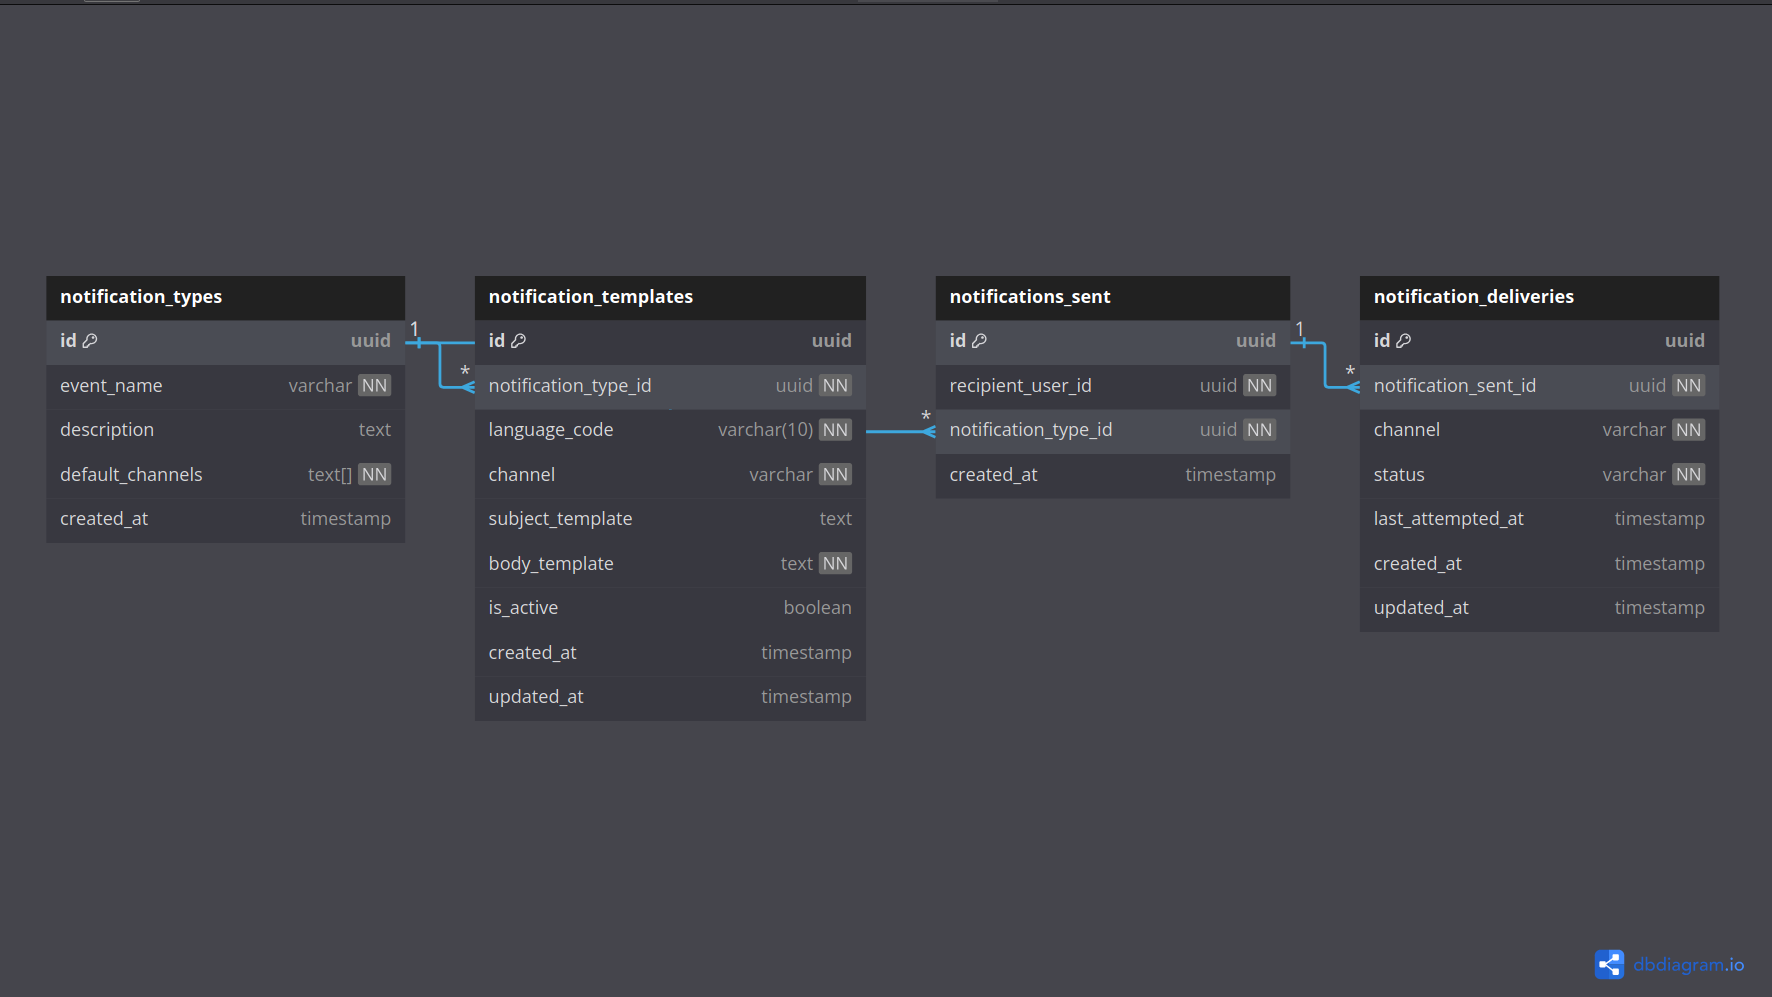
\includegraphics[width=0.8\textwidth,keepaspectratio]{week_1_img/services_db_screanshots/Screenshot 2025-06-06 at 15-08-13 Notification_Service.pdf.png}
  \caption{\textbf{Modèle de données du service de notification} pour la gestion des alertes et communications.}
  \label{fig:notification_service}
\end{figure}

\vspace{5pt}
\small
\paragraph{Points clés du service de Notification :}
\begin{itemize}[leftmargin=*,noitemsep,topsep=0pt]
  \item \textbf{Types de notifications} variés (email, in-app, SMS, push)
  \item \textbf{Modèles personnalisables} pour chaque type de message
  \item \textbf{Suivi de statut} (envoyé, livré, lu)
  \item \textbf{Planification} et envoi différé
  \item \textbf{Préférences utilisateurs} pour le contrôle des communications reçues
\end{itemize}
\normalsize
\clearpage

\subsubsection{Service de Gestion des Médias}
\begin{figure}[p]
  \centering
  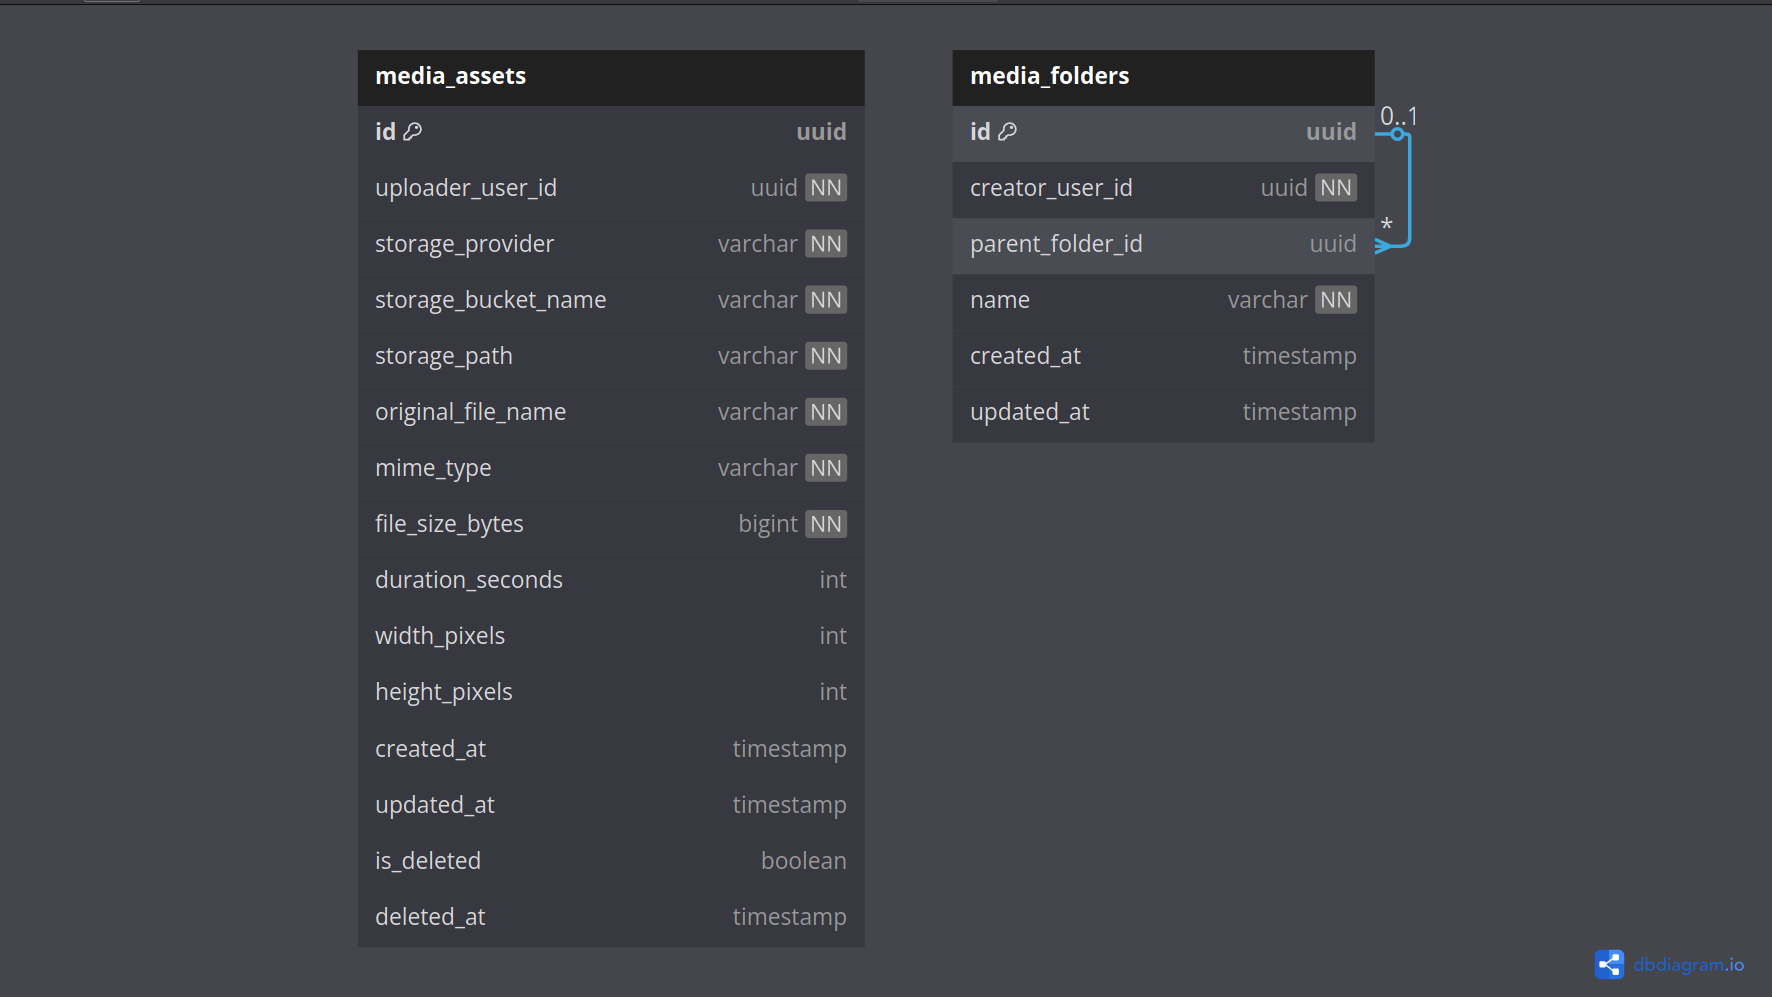
\includegraphics[width=0.8\textwidth,keepaspectratio]{week_1_img/services_db_screanshots/Screenshot 2025-06-06 at 15-08-27 Media_Management_Service.pdf.png}
  \caption{\textbf{Modèle de données du service de gestion des médias} pour le stockage et la manipulation des ressources multimédia.}
  \label{fig:media_service}
\end{figure}

\vspace{5pt}
\small
\paragraph{Points clés du service de Gestion des Médias :}
\begin{itemize}[leftmargin=*,noitemsep,topsep=0pt]
  \item \textbf{Organisation hiérarchique} des ressources multimédia
  \item \textbf{Métadonnées détaillées} pour faciliter la recherche et l'indexation
  \item \textbf{Versionnement} des fichiers pour garder l'historique des modifications
  \item \textbf{Gestion des transformations} (redimensionnement, compression, conversion)
  \item \textbf{Contrôles d'accès} pour sécuriser les ressources sensibles
\end{itemize}
\normalsize
\clearpage

\subsubsection{Service de Configuration de la Plateforme}
\begin{figure}[p]
  \centering
  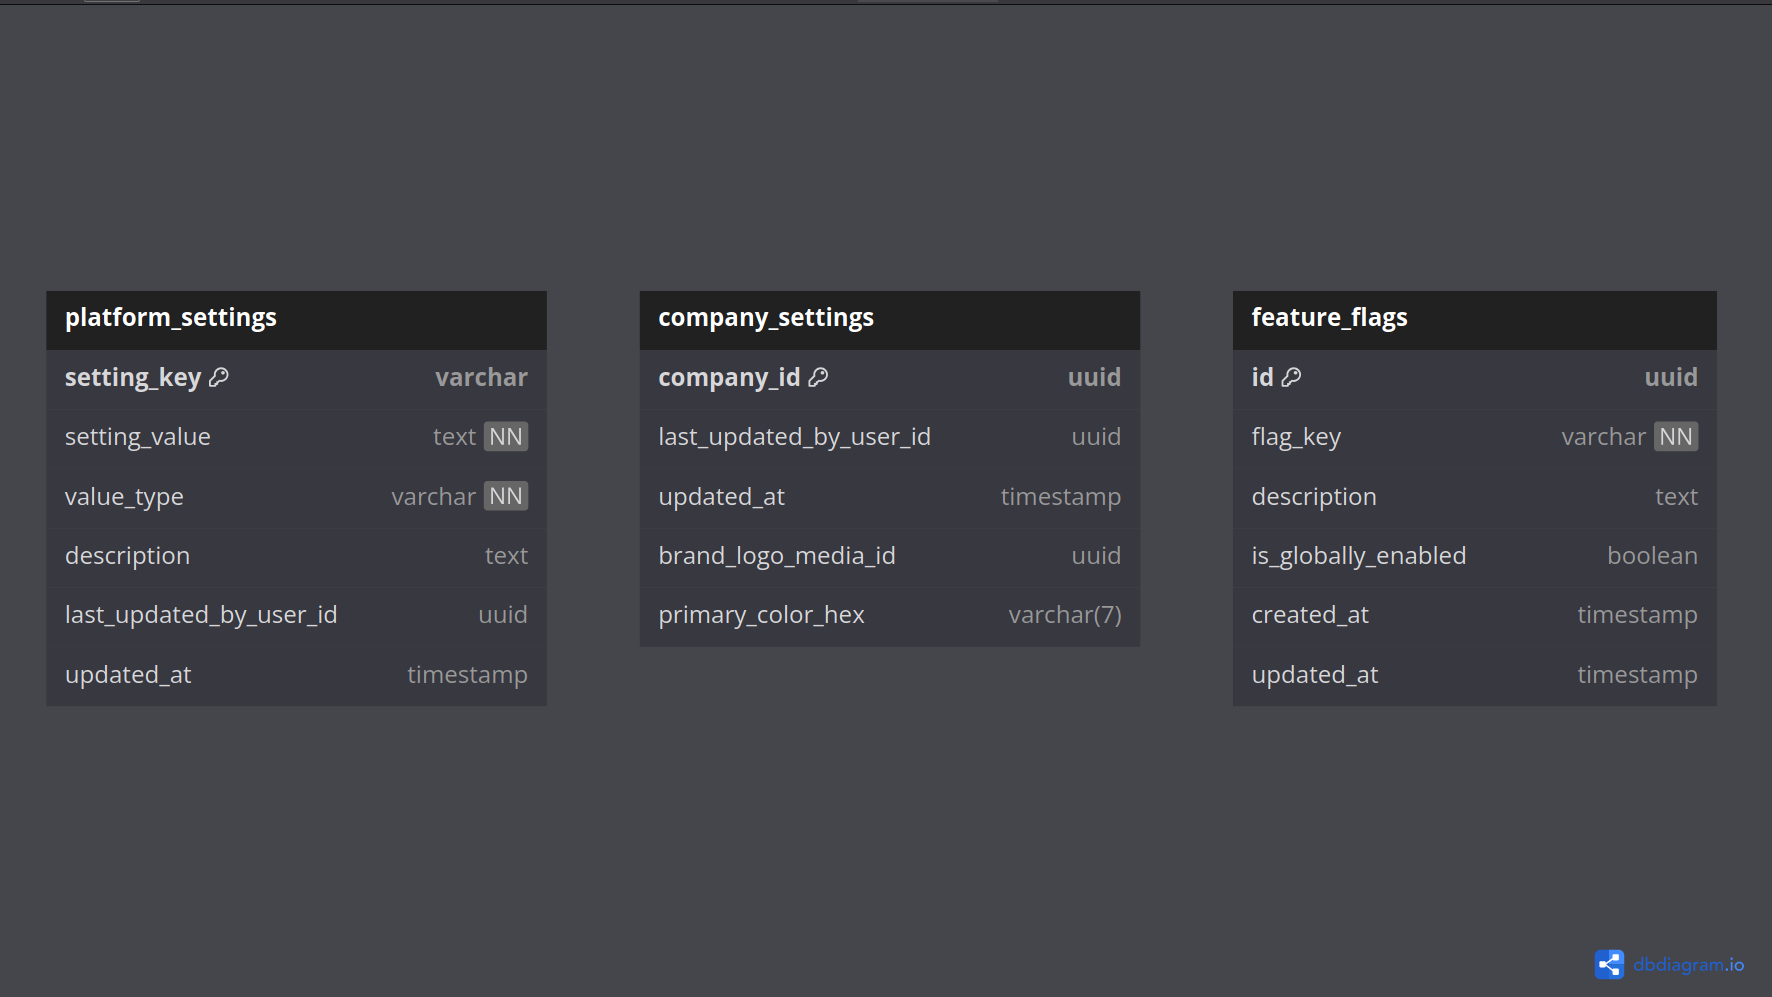
\includegraphics[width=0.8\textwidth,keepaspectratio]{week_1_img/services_db_screanshots/Screenshot 2025-06-06 at 15-08-44 Platform_Configuration_Service.pdf.png}
  \caption{\textbf{Modèle de données du service de configuration} pour la personnalisation et la gestion des paramètres de la plateforme.}
  \label{fig:config_service}
\end{figure}

\vspace{5pt}
\small
\paragraph{Points clés du service de Configuration :}
\begin{itemize}[leftmargin=*,noitemsep,topsep=0pt]
  \item \textbf{Paramètres système} pour contrôler le comportement de la plateforme
  \item \textbf{Personnalisation visuelle} (thèmes, couleurs, polices)
  \item \textbf{Fonctionnalités modulaires} activables/désactivables
  \item \textbf{Configuration multi-environnement} (dev, staging, production)
  \item \textbf{Historique des modifications} pour le suivi des changements
\end{itemize}
\normalsize
\clearpage

\subsubsection{Service de Recherche}
\begin{figure}[p]
  \centering
  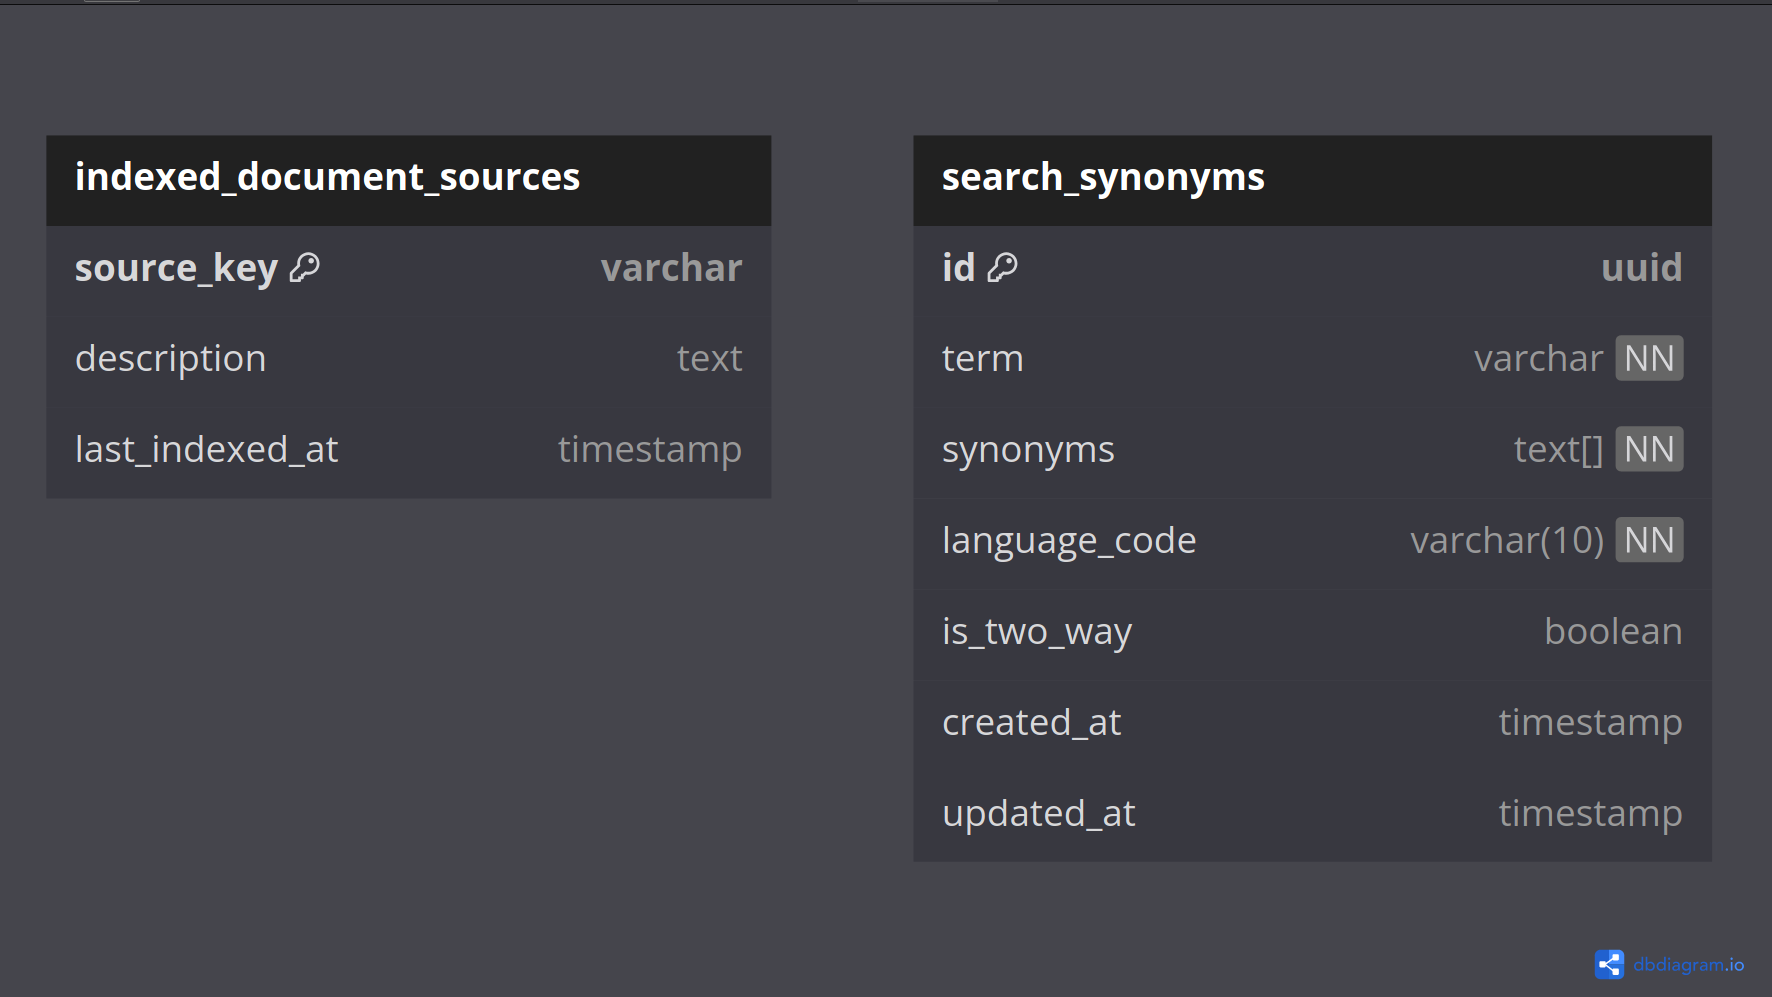
\includegraphics[width=0.8\textwidth,keepaspectratio]{week_1_img/services_db_screanshots/Screenshot 2025-06-06 at 15-08-52 Search_Service.pdf.png}
  \caption{\textbf{Modèle de données du service de recherche} pour l'indexation et la recherche de contenu.}
  \label{fig:search_service}
\end{figure}

\vspace{5pt}
\small
\paragraph{Points clés du service de Recherche :}
\begin{itemize}[leftmargin=*,noitemsep,topsep=0pt]
  \item \textbf{Indexation avancée} du contenu pour des recherches rapides
  \item \textbf{Filtres et facettes} pour affiner les résultats
  \item \textbf{Recherche full-text} avec correction orthographique
  \item \textbf{Optimisation sémantique} pour comprendre l'intention de recherche
  \item \textbf{Historique et suggestions} pour améliorer l'expérience utilisateur
\end{itemize}
\normalsize
\clearpage

\begin{table}[h!]
\centering
\small
\caption{Comparaison des caractéristiques techniques des services}
\label{tab:comparaison_services}
\begin{tabular}{|l|c|c|c|}
\hline
\textbf{Service} & \textbf{Technologie principale} & \textbf{Type de données} & \textbf{Complexité} \\
\hline
IAM & Node.js/Go & Utilisateurs & Élevée \\
Contenu & Python/FastAPI & Éducation & Moyenne \\
Facturation & Python/FastAPI & Financières & Élevée \\
Certification & Python/Go & Validation & Moyenne \\
Analytique & Python & Statistiques & Élevée \\
Feedback & Node.js & Évaluation & Basse \\
Notification & Go & Messaging & Moyenne \\
Médias & Node.js & Binaires & Élevée \\
Configuration & Go & Paramètres & Basse \\
Recherche & Python/Elasticsearch & Index & Élevée \\
\hline
\end{tabular}
\end{table}
\normalsize 

\section{Conclusion}

La conception et la modélisation de la plateforme LearnExpert ont été réalisées en adoptant une approche méthodique et structurée. Les différents diagrammes UML (cas d'utilisation, séquence, classes) ont permis de représenter visuellement les interactions, flux et relations qui forment l'ossature du système, fournissant ainsi une base solide pour les phases de développement ultérieures.

L'architecture microservices retenue offre plusieurs avantages stratégiques pour ce projet :
\begin{itemize}
  \item Une meilleure modularité, permettant l'évolution indépendante de chaque composant
  \item Une scalabilité granulaire, adaptée aux besoins variables de chaque service
  \item Une flexibilité technologique, avec l'utilisation des langages et frameworks les plus adaptés à chaque fonctionnalité
  \item Une robustesse accrue, grâce à l'isolation des défaillances potentielles
  \item Un développement parallèle facilité, permettant à différentes équipes de travailler simultanément
\end{itemize}

La modélisation détaillée des données pour chaque service constitue un élément clé de cette phase, avec une attention particulière portée à la cohérence, l'intégrité et l'efficacité des structures de données. La documentation minutieuse des schémas de base de données, des relations entre entités et des règles métier facilitera grandement la phase d'implémentation.

Cette étape de conception a également permis d'anticiper les défis techniques potentiels et de prévoir des solutions adaptées, notamment concernant la communication inter-services, la gestion des transactions distribuées et la sécurité des données. L'approche événementielle choisie, avec l'utilisation de Kafka comme broker de messages, offre un modèle de communication asynchrone particulièrement adapté à une architecture distribuée.

En conclusion, cette phase de conception a posé les fondations architecturales, conceptuelles et organisationnelles nécessaires au développement d'une plateforme e-learning moderne, évolutive et performante, alignée avec les objectifs définis dans le cahier des charges. 